\documentclass[runningheads]{llncs}
\usepackage{graphicx}
\title{\textbf{RGB Image Character Classification}}
\date{Dec-07-2018}
\author{Gihwan "Kris" Kwon\inst[1]}
\institute{University of Washington Bothell, Bothell WA 98011, USA\\
\email{kwonerstone3@gmail.com}\\}

\begin{document}
    \maketitle
    \pagenumbering{arabic}
    \begin{abstract}
        Machine learning in chracter recognition in images is popular research topics. It is well known that many machine learning
packages or models have been built to recognize characters in text or pdf files. Moreover, many research delved into recognizing
hand written characters or characters in natural images. It is rare to find any research focusing on recognizing characters in
'meme' images. Generally, memes contain digitally created characters in images. Searching memes from search engines rely on the
hash tag that uploader additionally uploaded. This paper focuses on recognizing digital character images, one by one. The model
is trained in convolutional neural networks and classify the character images. It explains the methods utilized to train and
analyzes the model from experimental results.
        \keywords{Convolutional Neural Networks \and Image Classification.}
    \end{abstract}

    \section{Introduction}
        Meme is a humorous image, video,
or piece of text that is copied and spread
rapidly by Internet users. Sometimes, people
want to search meme online and show it to their
friends that they liked. However,
often, it is hard to find the meme that a person
is looking for. Currently, online meme search engines are
relying on the hash tags to match user inputs with the results.
However, normally, users do not catch the phrase from the
hash tags, but the actual contents in the image. Therefore, it
would be useful to have meme search engines to have
an algorithm that can find the memes based on the word contents
inside the images.
\newline
\newline
\indent
Convolutional Neural Networks is a popular method to recognize images and
classify its label. Currently, there are many research focusing on utilizing
this method to recognize text images in real life. However, classifying
memes is different in that words in the memes are graphically added as contents.
Therefore, making a model for classifying graphically oriented characters
would be useful for developing search engines for memes.
\newline
\newline
\indent
The main goal of this project is to contribute to the developers who
would build a meme search engine for the users. To begin with, this project
will focus on classifying graphical characters. This paper will explain how
the model was built with the convolutional neural networking methods.


    \section{Method}
        The method used for this project is the Convolutional Neural Network.
This section explains methods for this project: Data preprocessing,
Training, Prediction.

        \subsection{Data Preprocessing}
            The original data sets are organized in the .csv file.
The objects are consist of attributes such as \textit{font} (string), \textit{fontVariant} (string), \textit{label}(int),
\textit{strength} (int), \textit{italic} (int), \textit{orientation} (int), \textit{m top} (int), \textit{m left} (int),
\textit{originalH} (int), \textit{originalW} (int), \textit{h} (int), \textit{w} (int), and 20 by 20 size grey scale image matrix.
Most of the attribute names are self-explanatory. However, to be more specific,
\textit{m top} and \textit{m left} are coordiate where image of the character starts in the real image in terms of row and column.
Moreover, \textit{originalH} and \textit{originalW} are original image size. Finally, \textit{h} and texit{w} are the height and weidth of
the image.
\newline
\newline
\indent
To begin with, some of the attributes are omitted in this process because recognizing font and whether the
character is italic are not the part of this project. Moreover, all the character images are original image.
In other words, image in the datasets only contains one character. Therefore, \textit{label} of the character and the
20 by 20 size grey scale image is going to be used in this project.
\newline
\newline
\indent
Next step is to convert the grey scale matrix into the RGB matrix which is three dimensional. The result matrix
after preprocessing would produce 20 by 20 by 3 image matrix. To be specific, conversion took place by appending
the original grey scale matrix into the result matrix three times. The result is the N number of RGB image matrices.
\newline
\newline
\indent
Furthermore, data preprocessing step produces a vector that values in each index contains character label and this
corresponds the image matrices stored in the image matrices. Finally, this step produces a matrix size of N by the number
of unique characters. The value in the indices are initially zeros in floating point. After image conversions, based on
the image label, vector for each image will contain 1.0 where index corresponds the image label. For instance, if there are
five different unique image labels in 10 different objects, the result will be ten by five matrix containing 1.0 in the vector
where index matches the character label, otherwise values will be 0.0s. In this case, the floating point one value specifies that
the index, character label, is true for corresponding image.
        \subsection{Training}
            The method of Convolutional Nerual Networks requires multiple layers in the process of trianing.
In a big picture, the layers could be divided into three layers: input, hidden, and output layers.
The input layer receives input, data such as matrices, and output layer produces the result values produced
by the model. Result values are N by the number of unique characters matrix that each vector contains the
probability of input to be the character of the corresponding index numbers. The layers are implemented while
utilizing the Tensorflow python package.
\newline
\newline
\indent
The hidden are further divided into three layers: Convolution, Flattening, and Fully Coonnected layers.

\paragraph{Convolution Layer}

\paragraph{Flattening Layer}

\paragraph{Fully Connected Layer}


    \section{Experiment and Result}
        This section will explain how the model was trained, validated, and tested. Several adjustments were
made to improve the model's prediction accuracy. For the training process, the model was trained with
training data sets and validated with validation data sets. On the other hand, testing data sets are
completely different from the training and validation data sets.
The number of training data sets are 47930 and validation sets are 5325. The validation set size is
roughly 10 percent of the training data sets. Five different experiment took place to improve the
prediction accuracy. In order to see the difference in the experiment, the model was trained with two
different learning rate and the number of epochs; Learning rate was 0.0001 and 0.00001; The number of
epochs are 17, 21, and 27. Finally, one batch of data sets contain 32 data sets.
\newline
\newline
\indent
To begin with, during the training process, the goal is to minimize the validation loss. Therefore,
training with different independent variables such as epoch sizes and learning rates produced the various
accuracy when predicting. The training processes and the results of prediction with the prediction accuracy are
provided in the figures below.
    \begin{figure}
        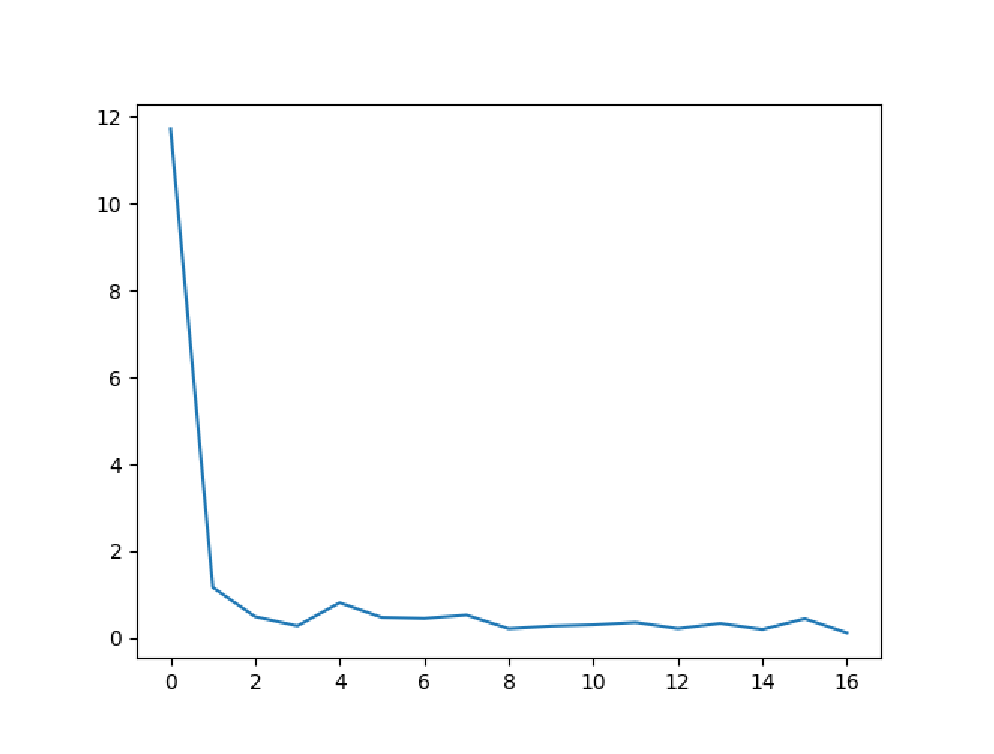
\includegraphics[width=\textwidth, scale=0.25]{4_25000.eps}
        \caption{Validation loss graph for epoch size 17 with learning rate 0.0001.} \label{Figure2}
    \end{figure}

    \begin{figure}
        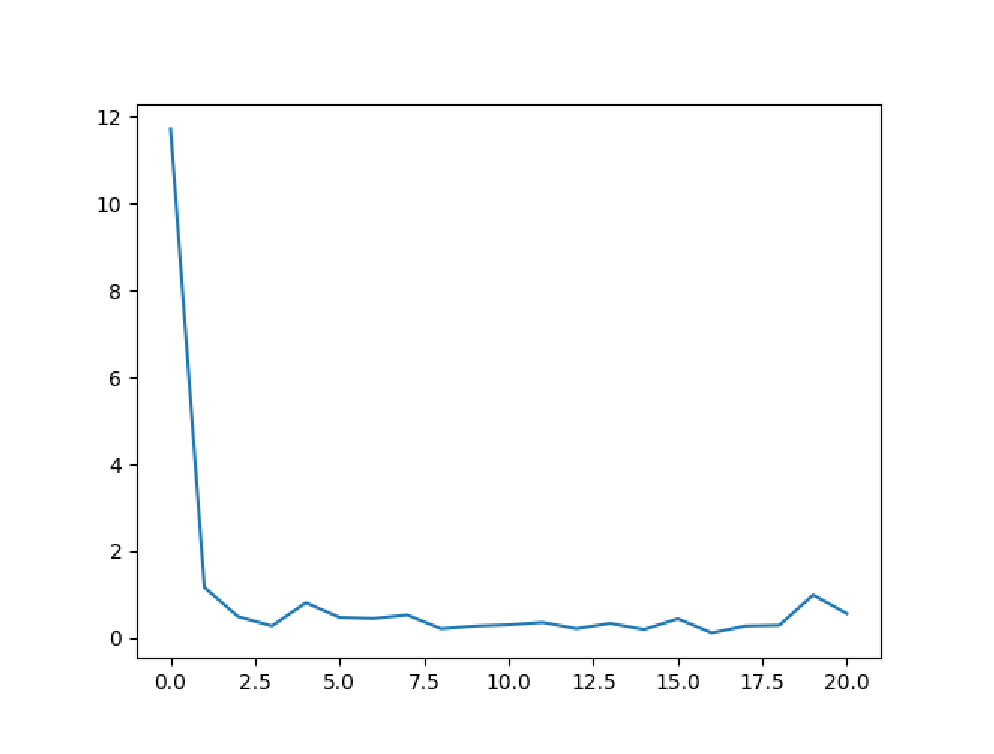
\includegraphics[width=\textwidth, scale=0.25]{4_30000.eps}
        \caption{Validation loss graph for epoch size 21 with learning rate 0.0001.} \label{Figure2}
    \end{figure}

    \begin{figure}
        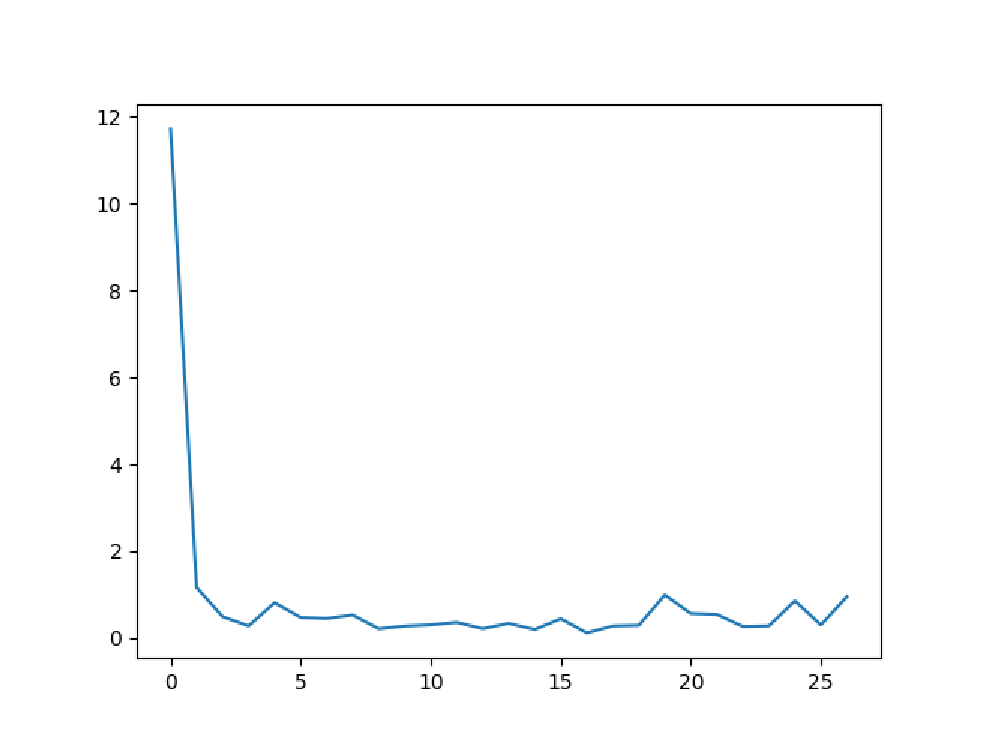
\includegraphics[width=\textwidth, scale=0.25]{4_40000.eps}
        \caption{Validation loss graph for epoch size 27 with learning rate 0.0001.} \label{Figure3}
    \end{figure}

Figures with learning rate of 0.0001 produces  with different number of iterations.
The first training seems

    \begin{figure}
    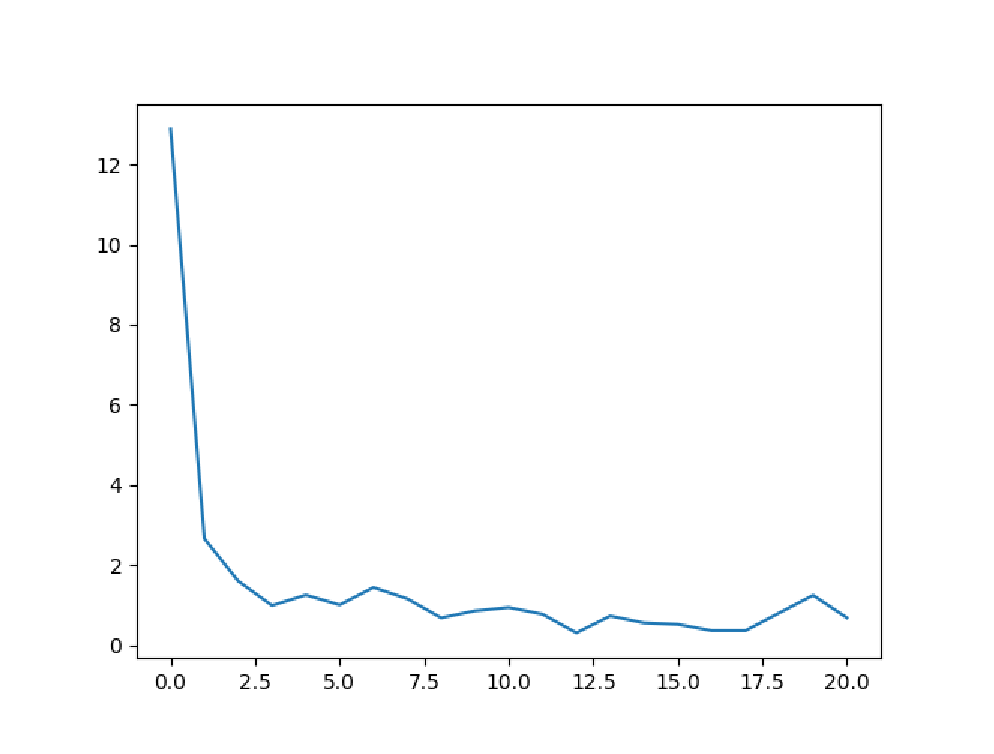
\includegraphics[width=\textwidth, scale=0.25]{5_30000.eps}
    \caption{Validation loss graph for epoch size 21 with learning rate 0.00001.} \label{Figure4}
    \end{figure}

    \begin{figure}
    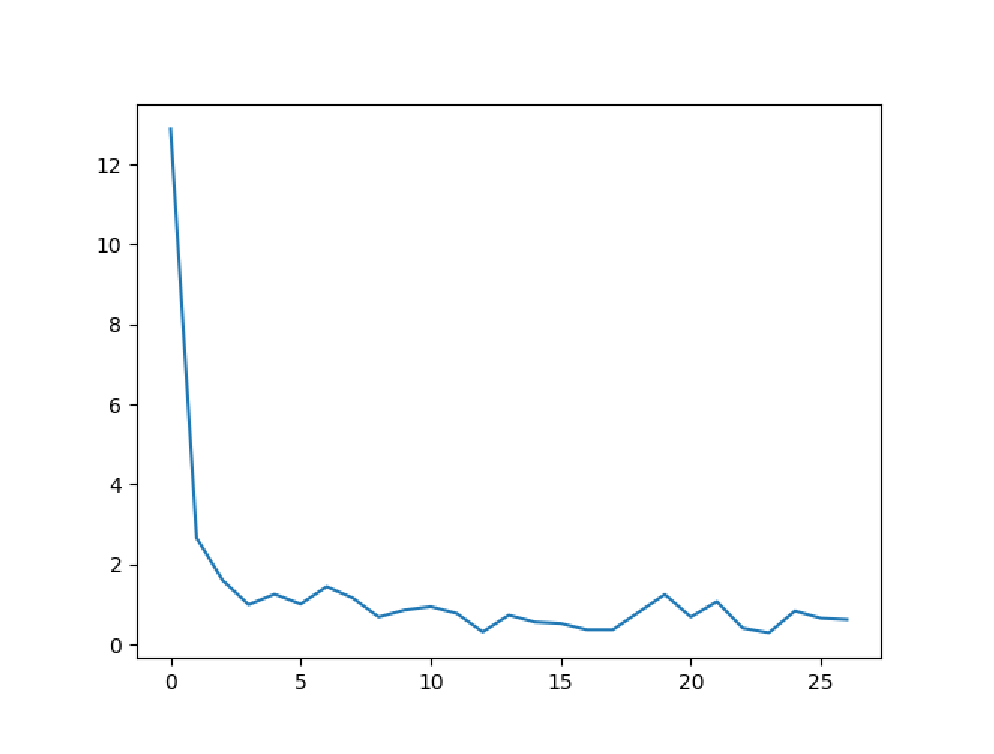
\includegraphics[width=\textwidth, scale=0.25]{5_40000.eps}
    \caption{Validation loss graph for epoch size 27 with learning rate 0.00001.} \label{Figure5}
    \end{figure}



        \paragraph{}
        \begin{figure}
        \includegraphics[width=\textwidth]{fig1.eps}
        \caption{A figure caption is always placed below the illustration.
        Please note that short captions are centered, while long ones are
        justified by the macro package automatically.} \label{fig1}
        \end{figure}
    \section{Conclusion}
        The purpose of this project was to classify characters in digital image. The model is trained and accurately predict the class
of character images. However, as mentioned, one of the challenges is to distinguish similar lower and upper case characters. This
challenge needs to be fixed in the stage of collecting input data or usage in applications. Moreover, the model can only predict
the one characters at a time. Recognizing phrases or sentences from 'memes' requires recognizing multiple characters. The future works
should focus on how to retrieve characters from 'memes' or utilizing this model for applications.
    \bibliographystyle{splncs04}
    \bibliography{references}

\end{document}